% ============================================================================
% Lecture 02 (B01): Why Deep Learning for Economics and Finance?
% Deep Learning for Solving and Estimating Dynamic Models in Economics and Finance
% Course author: Simon Scheidegger
% ============================================================================

\documentclass[aspectratio=169,11pt]{beamer}

% ---------- Theme and colors ----------
\usecolortheme{dove}
\setbeamertemplate{navigation symbols}{}
\setbeamertemplate{footline}{%
  \hfill\usebeamerfont{page number in head/foot}%
  \usebeamercolor[fg]{normal text}%
  \insertframenumber\,/\,\inserttotalframenumber\kern1em\vskip4pt}
\setbeamerfont{frametitle}{size=\huge}

% ---------- Packages ----------
\usepackage[utf8]{inputenc}
\usepackage[T1]{fontenc}
\usepackage{amsmath,amssymb,amsfonts}
\usepackage{bm}
\usepackage{graphicx}
\usepackage{tikz}
\usetikzlibrary{shapes,arrows.meta,positioning,calc,fit,backgrounds,patterns,decorations.pathreplacing}
\usepackage{pgfplots}
\pgfplotsset{compat=1.18}
\usepackage{booktabs}
\usepackage{hyperref}
\usepackage{multicol}
\usepackage{xcolor}
\usepackage{algorithm}
\usepackage{algorithmic}

% ---------- Custom colors ----------
\definecolor{uzhblue}{rgb}{0,0,0.5}
\definecolor{uzhgreylight}{RGB}{236,238,241}
\definecolor{uzhgreydark}{RGB}{81,86,94}
\definecolor{harvardcrimson}{RGB}{153,0,0}
\definecolor{unil@blue}{RGB}{0,140,204}
\definecolor{unil@black}{RGB}{35,31,32}
\definecolor{darkgreen}{RGB}{0,100,0}
\definecolor{darkred}{RGB}{139,0,0}
\definecolor{softblue}{RGB}{70,130,180}
\definecolor{softorange}{RGB}{230,159,0}
\definecolor{softgreen}{RGB}{0,158,115}

% ---------- Set beamer colors ----------
\setbeamercolor{frametitle}{bg=uzhgreylight, fg=uzhblue}
\setbeamercolor{title}{fg=uzhblue}
\setbeamercolor{structure}{fg=uzhblue}
\setbeamercolor{block title}{bg=unil@blue, fg=white}
\setbeamercolor{block body}{bg=uzhgreylight}
\setbeamercolor{block title alerted}{bg=darkred,fg=white}
\setbeamercolor{block body alerted}{bg=red!5}
\setbeamercolor{block title example}{bg=darkgreen,fg=white}
\setbeamercolor{block body example}{bg=green!5}
\setbeamercolor{item}{fg=unil@black}
\setbeamercolor{normal text}{fg=unil@black}

% ---------- Emphasis and hyperlinks ----------
\newcommand{\emphc}[1]{\textcolor{harvardcrimson}{#1}}
\hypersetup{colorlinks,linkcolor=harvardcrimson,urlcolor=harvardcrimson}

% ---------- Math commands ----------
\newcommand{\x}{\bm{x}}
\newcommand{\w}{\bm{w}}
\newcommand{\bb}{\bm{b}}
\newcommand{\z}{\bm{z}}
\newcommand{\W}{\bm{W}}
\newcommand{\X}{\bm{X}}
\renewcommand{\a}{\bm{a}}
\newcommand{\R}{\mathbb{R}}
\newcommand{\E}[1]{\mathbb{E}\!\left[#1\right]}
\DeclareMathOperator*{\argmin}{arg\,min}
\DeclareMathOperator*{\argmax}{arg\,max}

\title[Lecture 05 (B04)]{Lecture 05 (B04): Function Approximation and Loss Design}
\subtitle{Universal approximation, robust losses, the curse of dimensionality}
\author{Simon Scheidegger}
\institute{HEC, University of Lausanne}
\date{}
\begin{document}

{\setbeamercolor{background canvas}{bg=uzhgreylight}
\begin{frame}
\titlepage
\end{frame}
}

% --- About-this-lecture orientation ---
\begin{frame}{About this lecture}
\small
\begin{block}{What this lecture covers}
\begin{itemize}\itemsep2pt
  \item Universal approximation: what neural networks can and cannot represent
  \item Loss-function design beyond MSE: robust losses, asymmetric losses, choosing a loss
  \item Function approximation in moderate-to-high dimensions and the curse of dimensionality
\end{itemize}
\end{block}
\begin{block}{Builds on}
\begin{itemize}\itemsep2pt
  \item Lecture 03 (training mechanics)
  \item Lecture 04 (regularization)
\end{itemize}
\end{block}
\begin{block}{Leads to}
\begin{itemize}\itemsep2pt
  \item Lecture 06 (Deep Equilibrium Nets, where the loss IS the equilibrium residual)
\end{itemize}
\end{block}
\end{frame}

\begin{frame}{Universal Approximation Theorem}
\small
\begin{block}{Theorem (Cybenko 1989; Hornik, Stinchcombe \& White 1989)}
Let $g:\R\to\R$ be a bounded, non-constant, continuous activation function.  Then for any continuous function $f:\mathcal{K}\to\R$ on a compact set $\mathcal{K}\subset\R^d$ and any $\varepsilon>0$, there exists a single-hidden-layer network
\[
    F(\x) = \sum_{j=1}^{n_1} v_j\, g\!\big(\w_j^\top\x + b_j\big)
\]
such that $\sup_{\x\in\mathcal{K}} |F(\x) - f(\x)| < \varepsilon$.
\end{block}

\vspace{0.25cm}
\textbf{Caveats:}
\begin{itemize}\itemsep0pt
    \item The required width $n_1$ may be \textbf{exponentially large} in $d$.
    \item Existence $\neq$ efficient learnability.
    \item Practical success of deep learning suggests that \textbf{depth} provides a much more efficient parameterization than width alone.
\end{itemize}
\end{frame}
\begin{frame}{}
\begin{center}
{\Huge \textcolor{uzhblue}{Part III}}\\[0.8em]
{\LARGE Training: Loss, Gradients, and Optimization}
\end{center}
\end{frame}
\begin{frame}{Loss Functions}
The loss function $J(\bm{\theta})$ measures how far predictions $\hat{\bm{y}}$ are from targets $\bm{y}$.

\vspace{0.4cm}
\begin{columns}[T]
\column{0.48\textwidth}
\begin{block}{Regression: Mean Squared Error}
\[
    J(\bm{\theta}) = \frac{1}{2n}\sum_{i=1}^{n}\big(y^{(i)} - f(\x^{(i)};\bm{\theta})\big)^{2}
\]
Penalizes large deviations quadratically.
\end{block}

\column{0.48\textwidth}
\begin{block}{Classification: Cross-Entropy}
{\small
\[
    J = -\frac{1}{n}\sum_{i=1}^{n}\!\Big[y^{(i)}\!\log\hat{y}^{(i)} + (1{-}y^{(i)})\log(1{-}\hat{y}^{(i)})\Big]
\]}%
\vspace{-0.3cm}

For binary labels $y\in\{0,1\}$.
\end{block}
\end{columns}

\vspace{0.3cm}
\textbf{Multiclass} ($K$ classes): use softmax output $\hat{y}_k = e^{z_k}\big/\sum_j e^{z_j}$ and categorical cross-entropy:
$J = -\frac{1}{n}\sum_{i}\sum_{k} y_k^{(i)}\log \hat{y}_k^{(i)}$.
\end{frame}

% --- Slide 28a: Beyond MSE ---
\begin{frame}{Beyond MSE: Robust and Asymmetric Losses}
\begin{columns}[T]
\column{0.50\textwidth}
{\small
Let $r = y - \hat{y}$ denote the residual.

\vspace{0.1cm}
\textbf{MAE (L1):}\quad robust to outliers (constant gradient)
\vspace{-0.15cm}
\[
    L_{\text{MAE}} = \tfrac{1}{n}\textstyle\sum_{i=1}^{n}\big|r^{(i)}\big|
\]

\vspace{-0.25cm}
\textbf{Huber ($\delta$):}\quad smooth near zero, linear in the tails
\vspace{-0.15cm}
\[
    L_\delta(r) = \begin{cases} \tfrac{1}{2}r^2 & |r|\le\delta \\[2pt] \delta\!\left(|r|-\tfrac{\delta}{2}\right) & |r|>\delta\end{cases}
\]

\vspace{-0.25cm}
\textbf{Quantile / Pinball ($\tau\!\in\!(0,1)$):}
\vspace{-0.15cm}
\[
    L_\tau(r) = \begin{cases} \tau\,|r| & r \ge 0 \;\;(\text{under-predict})\\[2pt] (1{-}\tau)\,|r| & r < 0 \;\;(\text{over-predict})\end{cases}
\]

\vspace{-0.25cm}
$\tau{>}0.5$: penalises under-prediction more $\Rightarrow$ predicts \emph{high} quantile.
Directly gives VaR at level $\tau$.
}%

\column{0.46\textwidth}
\begin{center}
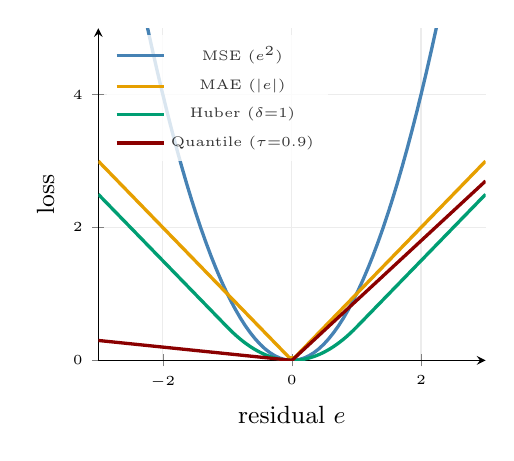
\begin{tikzpicture}
\begin{axis}[
    width=6.5cm, height=5.8cm,
    xlabel={residual $e$},
    ylabel={loss},
    xlabel style={font=\small},
    ylabel style={font=\small},
    tick label style={font=\tiny},
    xmin=-3, xmax=3, ymin=0, ymax=5,
    grid=major, grid style={gray!15},
    axis lines=left,
    legend style={font=\tiny, at={(0.02,0.98)}, anchor=north west,
                  row sep=1pt, draw=none, fill=white, fill opacity=0.8},
]
    % MSE: e^2
    \addplot[very thick, softblue, domain=-3:3, samples=80]{x^2};
    \addlegendentry{MSE ($e^2$)}
    % MAE: |e|
    \addplot[very thick, softorange, domain=-3:3, samples=80]{abs(x)};
    \addlegendentry{MAE ($|e|$)}
    % Huber (delta=1) — softgreen for high contrast against darkred Quantile
    \addplot[very thick, softgreen, domain=-3:-1, samples=40]{abs(x) - 0.5};
    \addplot[very thick, softgreen, forget plot, domain=-1:1, samples=40]{0.5*x^2};
    \addplot[very thick, softgreen, forget plot, domain=1:3, samples=40]{abs(x) - 0.5};
    \addlegendentry{Huber ($\delta{=}1$)}
    % Quantile (tau=0.9)
    \addplot[very thick, darkred, domain=-3:0, samples=40]{-0.1*x};
    \addplot[very thick, darkred, forget plot, domain=0:3, samples=40]{0.9*x};
    \addlegendentry{Quantile ($\tau{=}0.9$)}
\end{axis}
\end{tikzpicture}
\end{center}
\end{columns}
\end{frame}

% --- Slide 28b: Choosing a Loss Function ---
\begin{frame}{Choosing a Loss Function}
\begin{center}
{\small
\renewcommand{\arraystretch}{1.4}
\begin{tabular}{lcccc}
\toprule
\textbf{Loss} & \textbf{Outliers} & \textbf{Smoothness} & \textbf{Symmetry} & \textbf{Use case} \\
\midrule
MSE      & High & Smooth          & Symmetric           & Default regression \\
MAE      & Low  & Non-smooth at 0 & Symmetric           & Median regression \\
Huber    & Low  & Smooth          & Symmetric           & Robust regression \\
Quantile & Low  & Non-smooth at 0 & \textbf{Asymmetric} & Risk, VaR, tails \\
\bottomrule
\end{tabular}
}%
\end{center}

\vspace{0.5cm}
\begin{alertblock}{Why this matters in economics and finance}
Tail risks are often more important than average performance.
\textbf{Quantile loss} lets the model focus on getting worst-case predictions right,
directly producing Value-at-Risk (VaR) or Expected Shortfall estimates.
See \textbf{Notebook~07} for a hands-on comparison.
\end{alertblock}

\vspace{0.2cm}
{\small \textbf{References:} Huber (1964), Koenker \& Bassett (1978).}
\end{frame}
\begin{frame}{Exercise: Function Approximation with Neural Networks}
\textbf{Task:} approximate the Genz (1987) test functions with neural networks.

\vspace{0.2cm}
\begin{footnotesize}
\begin{align*}
    f_1(\x) &= \cos\!\Big(2\pi w_1 + \textstyle\sum_{i=1}^{d} c_i x_i\Big) & &\text{(oscillatory)} \\
    f_2(\x) &= \textstyle\prod_{i=1}^{d} \big(c_i^{-2} + (x_i - w_i)^2\big)^{-1} & &\text{(product peak)} \\
    f_3(\x) &= \Big(1 + \textstyle\sum_{i=1}^{d} c_i x_i\Big)^{-(d+1)} & &\text{(corner peak)} \\
    f_4(\x) &= \exp\!\Big(-\textstyle\sum_{i=1}^{d} c_i^2(x_i - w_i)^2\Big) & &\text{(Gaussian)} \\
    f_5(\x) &= \exp\!\Big(-\textstyle\sum_{i=1}^{d} c_i|x_i - w_i|\Big) & &\text{(continuous)} \\
    f_6(\x) &= \begin{cases}0 & \text{if } x_1>w_1 \text{ or } x_2>w_2\\ \exp\!\big(\textstyle\sum_{i=1}^{d}c_i x_i\big) & \text{otherwise}\end{cases} & &\text{(discontinuous)}
\end{align*}
\end{footnotesize}

\vspace{0.1cm}
{\small Pick 3 functions. Train NNs on 10, 50, 100, 500 random points from $[0,1]^d$.  Compute average and max error on 1000 test points.  Repeat for $d\in\{2,5,10\}$.}
\end{frame}

% --- Slide 53: Questions ---
\begin{frame}{}
\begin{columns}[c]
\column{0.45\textwidth}
\begin{center}

\includegraphics[width=0.85\textwidth]{figures/quest.png}
\end{center}

\column{0.50\textwidth}
\begin{center}
{\Huge \textcolor{uzhblue}{\textbf{Questions?}}}

\vspace{0.8cm}
{\large Simon Scheidegger}\\[4pt]
{\small HEC, University of Lausanne}\\[4pt]
\url{https://sischei.github.io}

\vspace{0.6cm}
{\small Materials:~~\url{https://github.com/sischei/Deep_Learning_for_Solving_And_Estimating_Dynamic_Economic_Models}}
\end{center}
\end{columns}
\end{frame}

\end{document}
